\documentclass[sigconf]{acmart}

\usepackage{booktabs} % For formal tables
\usepackage{tikz,pgfplots}

\begin{document}
\title{PyPandas: A data cleaning toolkits for Spark}

\author{Pei-Lun Liao}
\affiliation{%
  \institution{New York University}
}
\email{pll273@nyu.edu}

\author{Chia-Hsien Lin}
\affiliation{%
  \institution{New York University}
}
\email{chl566@nyu.edu}

\author{Shang-Hung Tsai}
\affiliation{%
  \institution{New York University}
}
\email{st3127@nyu.edu}

\begin{abstract}
Data cleaning is a huge challenge in data mining and machine learning tasks. In this paper, we propose PyPandas, a data cleaning toolkits running on Spark, to provide further solutions to data cleaning tasks. PyPandas provides advance cleaning features such as outlier detection, data scaling and text pattern searching and replacement. We have released PyPandas on GitHub\footnote{https://github.com/shtsai7/PyPandas} and Python Package Index (PyPI).\footnote{PyPandas can be installed by pip.}
\end{abstract}

\maketitle

\section{Introduction}
In recent years, as storage devices become cheaper, storing big data in thousands of computers is easier than before. People start thinking about how to extract useful information from the huge datasets. The term, Big Data, was created to describe this phenomenon\cite{bigdata}. As the result, data mining\cite{Han, MMD} and machine learning\cite{ml} get popular nowadays. The quality of data is one of the key factors to successful data mining\cite{dataquality}. Hence, data cleaning becomes a challenge in the first step of data management and analysis\cite{datacleaning, DBS-045, PW}.
	
To process huge datasets efficiently, distributed systems and parallel computing frameworks\cite{mapreduce, gfs, hadoop} were introduced. Spark\cite{spark} is one of the most popular open source projects for industry and academia. It is built on Hadoop\cite{hadoop} and provides a way to manage distributed memory. PySpark\cite{pyspark} is an extended library for Python programmers to work with Spark.
	
In the Python machine learning and data mining ecosystem, Pandas\cite{pandas} is the most popular data management library. Pandas dataframe provides convenient ways to collect data and several data management methods for missing value filling, data indexing and data profiling. In PySpark SQL module, PySpark provides Pandas-liked DataFrame to handle data indexing, data integration, and simple data cleaning tasks such as missing value handling and duplication removal.
	
However, PySpark DataFrame does not support advance data processing features like outlier detection and data scaling. Although there exists several clustering and scaling algorithms in the PySpark ML module, the integration with PySpark DataFrame is not helpful and can be difficult to use for data cleaning. User has to go back and forth to process their dataset.  

In this paper, we propose PyPandas, a data cleaning toolkits built on top of PySpark, that integrates PySpark ML module to support user friendly data processing features such as outlier detection and numerical data scaling. These features are important for the machine learning tasks and are supported in Scikit-Learn\cite{scikit-learn}, a mainstream machine learning library, as well.
	
Furthermore, text data is another common data type in our storage. Text data is hard to process because of different languages, newly invented words, typos, abbreviations, urls and emoji etc.  In this paper, we also implement easy to use text cleaning methods and provide flexibility for users to customize their cleaning processing. 
	
The features of our library are summarized below.
\begin{itemize}
	\item{User friendly data cleaning toolkits built on PySpark}
	\item{Outlier detection and numerical data scaling}
	\item{Text processing such as url detection, punctuation removing, pattern searching and replacement. }
\end{itemize}	

\section{Related Work}
There exists a number of open-source library for data cleaning and parallel data computing. 
\begin{itemize}
	\item{Optimus}\cite{optimus} is a framework that can perform distributed data cleaning and preprocessing. This framework works well with Spark and its DataFrame can scale in big cluster. Optimus comes with helpful tools such as removing special characters and replacing null values.
	\item{Dask}\cite{dask} is another open-source library that supports parallel analytic computing. It provides scalable parallel data structures that extend interfaces like Pandas. At the same time, it offers low latency and high responsiveness.
	\item{SparklingPandas}\cite{sparklingpandas} attempts to combine the power of Spark and Pandas to scale data analysis. It provides a Pandas-like API that is built using Spark's DataFrame class. Unfortunately, it only support spark v1.4 and Python 2.7, and its development has ended.
\end{itemize}

\section{Problem Formulation}
In this paper, we focus on three major tasks, outlier detection, data scaling, and text pattern searching and replacement.
\subsection{Outlier Detection}
Outlier or anomalies detection is a challenging task in the field of data cleaning\cite{anomal}. In this paper, we define outlier as the data that is far away from the its cluster centroid. Hence, given a dataset $X$, a clustering algorithm $A$\cite{MMD}, a distance measurement $d$, and the user-defined threshold $t$, the outlier is defined as following.

\[ outlier = \{x | x \in X, d( x, c_{A_X(x)} ) > t \}  \]

where $A_X(x)$ assigns $x$ into a cluster given the dataset $X$ and $c_{A_X(x)}$  is the centroid of cluster to which $x$ belongs.
Our library implements the following clustering algorithms. 
\begin{itemize}
	\item{K-Means and Bisecting K-Means Algorithm}\cite{KMeans, biKmeans} \\
		These two algorithms partition data points into k clusters, where each point belongs to the clusters that is closest to that point. In these two models, the distance measurement $d$ is the Euclidean Distance.
		\[ d( x, c_{KMeans_X(x)}) = \sqrt{\sum_{i=1}^n{(x_i - c_i ) ^ 2} } \]
	\item{Gaussian Mixture Model}\cite{GMM} \\
		The algorithm assumes a probabilistic model where data points are generated from some Gaussian distributions. The Gaussian distributions are parameterized by a mean $\vec{\mu}$ and a covariance matrix $S$.
		The distance measurement $d$ is defined to be Mahalanobis Distance, which measures the distance between a point and a distribution.
		\[ d( x, c_{GMM_X(x)}) = \sqrt{(\vec{x}-\vec{\mu})^T S^{-1} (\vec{x}-\vec{\mu}) } \]
\end{itemize}

\subsection{Scaling and Normalization}
Scaling and normalization are common preprocess in data cleaning. It is crucial to several machine learning models and optimization methods. Scaling increases the convergence speed and chance to find good optimum\cite{convex}. The scaling problem could be formulated as below.
Given an one dimensional numerical dataset $X$, we provide a scaling method $S$ such that scaled elements are bounded in same reasonable range $[a, b]$.

\[ S_X(x) \in [a, b]\] 

where $x \in X$ and $|a - b|$ should not be large.

To define the problem formally, we consider and implement several specific scaling methods.
\begin{itemize}
	\item{Standard scale}
		\[ S(X) = \dfrac{X-\mu}{\sigma} \in \text{proper deviation range}\]
		where $\mu$ is the mean of $X$ and $\sigma$ is the standard deviation of $X$
	\item{Min-Max scale}
		\[ S(X) = \dfrac{X-min(X)}{max(X) - min(X)}\in [0.0, 1.0] \]
	\item{Max-Abs scale}
		\[ S(X) = \dfrac{X}{max(X)} \in [-1.0, 1.0] \]
	\item{P-norm Normalization}
		\[ S(X) = \dfrac{X}{\|X\|_{p}} \in [-1.0, 1.0]\]
\end{itemize}

\subsection{Pattern Searching and Replacement}
Pattern searching and replacement is a common technique in cleaning text data. Given a string $t$ and a regular expression\cite{theory_com} $re$, we replace the matched pattern with a user-defined string $s$. The replacement function $R$ could be defined as following.
Consider $t$ as a concatenation of non-overlapping substrings $t = t_1...t_n$.

\[ R(t) =  r(t_1)...r(t_i)...r(t_n)\]

\[r(t) = \begin{cases} s & \text{if $M$ accept $t$} \\ t & \text{otherwise} \end{cases}\]

\[\text{such that $M$ does not accept any substring of } R(t)\]

where $M$ is the generalized nondeterministic finite automaton\cite{theory_com} corresponding to the regular expression $re$. We do not define replacement order and simply ignore it.


\section{Methods, Architecture and Design}
In this project, we build our library on top of PySpark. We handle PySpark DataFrame and implement useful data cleaning functions in our library. We integrate PySpark ML module and customize user define functions to perform advanced cleaning features such as pattern searching and replacement with regular expression. We survey the PySpark\cite{pyspark}, Pandas\cite{pandas} and Scikit-Learn\cite{scikit-learn} libraries to find out key features and create Pandas-like and Scikit-Learn-like API to provide easy usage and seamless adaptation.

\subsection{Outlier Detection}
\subsubsection{Design} 
Our goal in outlier detection is to integrate the existing clustering algorithms in PySpark ML module to provide user-friendly solution for outlier detection. Users are able to select existing clustering algorithms. Furthermore, users are given the power to decide their own threshold value based on their knowledge about the dataset to filter outliers. To help users identify outliers and pick a proper threshold, we provide statistics summary of the clustering. 
%Possible future work on outlier detection is to provide framework to register user defined clustering algorithms or implementing popular clustering algorithms such as DBScan\cite{DBScan} in our library.

\subsubsection{Architecture}
The implementation of the outlier detection functionality integrates the PySpark ml package. Our architecture hides the complexity of training and tuning clustering models, while it exposes easily accessible APIs for users to remove outliers. In addition, our data cleaning library implements User Defined Functions to compute distance between data points and cluster centers, as well as other summary statistics. At this time, our outlier remover can handle outliers with KMeans clustering, Bisecting KMeans, and Gaussian Mixture Model. We use Factory Design Pattern to construct different types of outlier removers with the generic APIs.

\subsubsection{Methods}
\begin{itemize}
	\item{KMeans}\cite{KMeans}: Users can specify the number of clusters $k$ to use based their knowledge about the dataset. By default, The system will choose random initial values, and perform 20 iterations of updates. Finally, a summary of the clusterings will be generated, which includes cluster centers, cluster sizes, distances, etc. User can then filter out outliers in each cluster by specifying a minimum distance from the cluster center, and all data points that are beyond that distance will be removed from the dataset.
	\item{Bisecting KMeans}\cite{biKmeans}: Bisecting Kmeans clustering algorithm is similar to KMeans. However, the algorithm does not start with k clusters. Instead, it gradually divides clusters and generates k clusters after a number of iterations.
	\item{Gaussian Mixture}\cite{GMM}: Similarly, users can specify the number of clusters (i.e. Gaussian distributions). The algorithm performs 20 iterations of updates by default. A summary that contains mean, covariance matrix and average mahalanobis distance of each cluster can be returned. User can specify a minimum distance to filter out outliers.

\end{itemize}

\subsection{Scaling and Normalization}
\subsubsection{Design}
Standardization is a common requirement for many machine learning algorithms, since some optimization methods will not work properly without scaling or normalization\cite{convex}. Our goal in scaling and normalization is similar to the goal of outlier detection. We will intergrate existing scaling algorithms in PySpark ML module into our library. User can choose existing scaling algorithms to scale their datasets. %The future works is to provide framework to register user defined scaling algorithms.

\subsubsection{Architecture}
The architecture of scaling is simple. We wrap scaling logic into single function which allows user to transform their PySpark DataFrame easily.
%Since the design is similar with the design of outlier detection, we will follow the architecture of outlier detection. We will use the Factory Design Pattern to allow users construct their desired scaling models. We are considering to implement a single interface between any existing models in PySpark ML module to DataFrame in PySpark SQL module. Hence, we will be able to provide any feature transformation with the existing machine learning models in PySpark ML module.

\subsubsection{Methods}
\begin{itemize}
	\item{Standard Scale}: Performs basic scaling on a particular column or a list of columns in a dataframe so that the values have unit standard deviation and zero mean. 
	\item{Min-max Scale}: Rescales columns to a user defined range(e.g. [0, 1]) using min max scaling.
	\item{Max-abs Scale}: Transforms columns to range between -1 and 1 by dividing through the maximum absolute value in the columns. This operation does not shift/center the data, and thus does not destroy any sparsity. 
	\item{Normalization}: Given a list of columns, the normalize function can generate a normalized feature vector having unit norm. The default p-norm value for normalization is 2.0, yet users can optionally specify the p-norm value.
\end{itemize}

\subsection{Pattern Searching and Replacement}
\subsubsection{Design} 
To provide a useful text cleaning toolkits, we need to have the flexibility for user to search any pattern and replace the matched ones with any user defined string. At the same time, we have to provide common patterns so that users won't need to reinvent the wheel. For example, url pattern, leading space, trailing space or numbers are common search patterns that we should provide. Moreover, users should be able to organize their cleaning logic and apply them to the text dataset easily.%Moreover, we would like to integrate NLTK\cite{nltk}, a popular natural language toolkit, into our library. With NLTK, we would be able to perform advanced cleaning tasks or feature transformation.
%%to follow the don't repeat yourself (DRY) principle 

\subsubsection{Architecture}
In order to achieve those design issues, we extract the common logic and column feature transformation into our core functions. We design the architecture such that user defined functions can be applied on a single or multiple columns, and a new DataFrame will be provided. The user defined function could be a regular expression substitution function, a column scaling function or a natural language processing function in NLTK\cite{nltk}. Our architecture ensures the flexibility to various customized processing methods. Futhermore, we apply Decorator Design Pattern to enable users to register processing functions and customize their cleaning process.

\subsubsection{Methods}
We define several common regular expression patterns in table \ref{tab:reg} and provide simple cleaning functions to handle those patterns in text data.
\begin{table}
\caption{Common Regular Expression Pattern}   
\label{tab:reg}
\begin{tabular}{lc}
	Common Pattern & Regular Expression \\
\hline
	URL & URL regular expression\cite{url} \\
	Leading space & \verb!'^ +'! \\
	Trailing space & \verb!' +$'! \\
	Consecutive space & \verb!' +'! \\
	Number & \verb!'\d+'!  \\
	Not a word & \verb!'[^\w\d\s]+'! \\
	Blank & \verb!'_+'!
\end{tabular}   
\end{table}

\begin{table}
\caption{Selected dataset}   
\label{tab:dataset}
\begin{tabular}{lccc}   
 		                 & (Row, Col)  & Size      & Property  \\  
\hline
 311 Service Requests    & (9M, 53)     & 6.01 GB  & Text            \\ 
 Permit Issuance            & (3M, 60)     & 1.43 GB  & Mixed Type \\  
 Job Application Filings   & (5M, 89)      & 2.88 GB  & Numerical Value      \\ 

\end{tabular}   
\end{table}

\begin{table*}
\caption{Evaluation: Features Comparison}   
\label{tab:features}
\begin{tabular}{lccccc}
						&  PySpark DataFrame\cite{pyspark} 	& PyPandas 	& Optimus\cite{optimus} 	& SparkingPandas\cite{sparklingpandas} 	& Dask\cite{dask}	\\
&&&&& \\
Data manipulation &&&&& \\
\hline
Data integration				& \checkmark 	        			& \checkmark   	& \checkmark		& 							& \checkmark	 \\
Data aggregation				& \checkmark 	        			& \checkmark   	& \checkmark		& \checkmark					& \checkmark	 \\
Data filtering					& \checkmark 	        			& \checkmark   	& \checkmark		& 							& \checkmark	 \\
Data profiling				& \checkmark 	        			& \checkmark   	& \checkmark		& \checkmark					& \checkmark	 \\
Data sorting					& \checkmark 	        			& \checkmark   	& \checkmark		& 							&	 		 \\

&&&&& \\
Basic data cleaning &&&&& \\
\hline
Missing value filling	 			& \checkmark 		  	      	& \checkmark   	& \checkmark		& 							& \checkmark	 \\
Missing value removing			& \checkmark 	 	  	     	& \checkmark   	& \checkmark 		& 							& \checkmark	 \\
Duplication removing 			& \checkmark 			       	& \checkmark 	& \checkmark		&							& \checkmark	\\	

&&&&& \\
Outlier Detection &&&&& \\
\hline
Deviation with median			&						& 			& \checkmark		&							&			\\
Clustering algorithms			&						& \checkmark	& 				&							&			\\	
	
&&&&& \\
Scaling and Normalization &&&&& \\
\hline
Standard scaling				&						& \checkmark	& 				&							& \checkmark	\\		
Scale in range				&						& \checkmark	& \checkmark		&							& \checkmark	\\
Normalization				&						& \checkmark	& \checkmark		&							& 			\\



&&&&& \\
Text Cleaning &&&&& \\
\hline
Special character removing		& \checkmark				& \checkmark	& \checkmark		&							&		\\
Pattern searching 			 	& \checkmark				& \checkmark	& \checkmark		&							&		\\		
Pattern searching and replacement 	&						& \checkmark	& \checkmark		&							&		\\
Common patterns replacement		&						& \checkmark	&				&							& 		\\
\end{tabular}
\end{table*}


\section{Experiment}
\subsection{Dataset}
Three datasets are chosen for the experiments. Each of them has different properties and can be used to test different parts of the library. The summary of datasets could be found in table \ref{tab:dataset}.
\begin{itemize}
	\item{311 Service Requests}\cite{nycopendata1} This dataset contains all 311 Service Requests since 2010. The majority of data has string type, including both categorical  data (e.g. City, Status) and variable length data (e.g. Address, Description). This can be useful in testing the string-related features of the library.
	\item{DOB Permit Issuance}\cite{nycopendata2} The dataset consists of a list of permits for buildings in NYC issued by Department of Building. It has diverse data types, including categorical, string, numerical, and geographical data. Hence, it provides a good test case for the versatility of the library. 
	\item{DOB Job Application Filings}\cite{nycopendata3} The dataset stores job applications filed through the Borough Offices in NYC. There are many columns containing numerical data, such as fee and number of stories. It can be used to test the data scaling and outlier detection features. 
\end{itemize}

\subsection{Evaluation}
We evaluate our project by comparing it against other existing open-source libraries, including Optimus\cite{optimus} and Dask\cite{dask}. In addition, we examine the scalability of the library.
\subsubsection{Features}
We compare our data cleaning features with previous works, particularly those frequently used functionality in data science such as null value handling, special character removal, duplicate detection, etc. 
\subsubsection{Performance}
We evaluate the performance of our library by measuring the time consumed and drawing comparison with existing libraries. This performance evaluation shows that this library is efficient and can be useful in production. 
\subsubsection{Scalability}
We examine the scalability of our library by running the same task with different numbers of worker nodes. We measure the time consumed under different configuration and analyze the scalability. This evaluation shows how well the library can scale.
%\subsubsection{Usability}
%We might assess the usability of our library by doing a survey among a random group of users. We will compare the installation process and APIs provided and generate scores of user experience.

\subsection{Results}
After running our experiments on the Dumbo clusters of NYU initially, we migrate all our settings to Amazon Web Service because we could not obtain the privileges needed on Dumbo. While on Amazon Web Service, we can obtain the privileges needed to install other packages and we are able to perform comparison with other related works. In addition, on Amazon Web Service, we are able to customize the clusters we need, such as setting the number of worker nodes. This allows us to perform the scalability experiments.

\subsubsection{Features}
In this section, we compare our features with previous works. The result is shown in table \ref{tab:features}. We find that PySpark DataFrame provide easy-to-use data manipulation functions. Since PyPandas and Optimus extend the DataFrame, both of them support the same data manipulation features. In SparkingPandas, the project only aims to provide grouping methods on Pandas-liked dataframe and miss other important features in data manipulation. Dask also support many features in data manipulation. 

PySpark DataFrame, Optimus, Dask, and our library PyPandas all provide the basic data cleaning functions like missing value handling. In the outlier detection, Optimus detects outliers by calculating the deviation with the median of data. On the other hand, PyPandas provides advance detection methods with clustering algorithms. Dask do support several clustering algorithms. Nonetheless, they are not integrated in their Dask DataFrame. Users have to manually train and tune the models to detect the outliers.

In scaling and normalization, Optimus, Dask and PyPandas provide basic scaling methods like min-max scaling. However, Dask does not provide normalization on their Dask ML preprocessing module. And Optimus does not support standard scaling.

For the text cleaning, Optimus and PyPandas provides more powerful pattern searching and replacement feature to let user find out any pattern and replace the matched one with their desired value. Moreover, PyPandas defines several common patterns for users to clean their text quickly without repeating themselves and users are able to register their cleaning logic to customize their process in text cleaning. In summary, PyPandas extends PySpark DataFrame and provides more easy-to-use features for users to clean their data.

\subsubsection{Performance} We compare the performance of functions including min max scaling, normalization and special character cleaning in our library against those in Optimus on AWS EMR with the identical environment configuration. The data processing time and total execution time, including the time for Spark initialization, data loading, and data processing, are all recorded and listed below. Even though the execution times seems to be slightly slower than Optimus, we do provide more features in PyPandas.

\begin{itemize}
	\item{Scaling and Normalization}: In this experiment, the min max scaling and the normalization are performed on the 311 Service Requests Dataset. We select all the numeric columns in the dataset to do the experiment. The experiment results can be found in table \ref{tab:Scaling and Normalization Experiment Result}.
	\item{Special Character Cleaning}: In this experiment, the special character cleaning is performed on the 311 Service Requests Dataset. We execute the cleaning function to the entire dataset. The results are shown in table \ref{tab:Special Character Cleaning Experiment Result}.
\end{itemize}

\begin{table}
\caption{Scaling and Normalization Experiment Result}   
\label{tab:Scaling and Normalization Experiment Result}
\begin{tabular}{lcc}   
 	         &  Min-Max Scaling  &  Normalization \\
\hline
PyPandas   &  319.08s / 391.11s  & 32.87s / 105.90s  \\ 
Optimus     &   85.24s / 142.46s   & 31.21s / 61.92s   \\
\end{tabular}
\end{table}

\begin{table}
\caption{Special Character Cleaning Experiment Result}   
\label{tab:Special Character Cleaning Experiment Result}
\begin{tabular}{lccc}   
                 & 311 Service  & Permit     & Job Application \\  
		 &	Requests  & Issuance  & Filings  \\ 
\hline
PyPandas   &  31.92s / 104.18s  & 10.29s / 62.35s   & 10.80s / 60.07s             \\ 
Optimus     & 32.32s / 86.19s    & 9.77s / 43.67s   & 10.35s / 43.04s             \\  
\end{tabular}   
\end{table}

\begin{figure}
\caption{Scalability Experiment - Outlier Detection}   
\label{plt:Outlier Detection - Scalability Experiment Result}
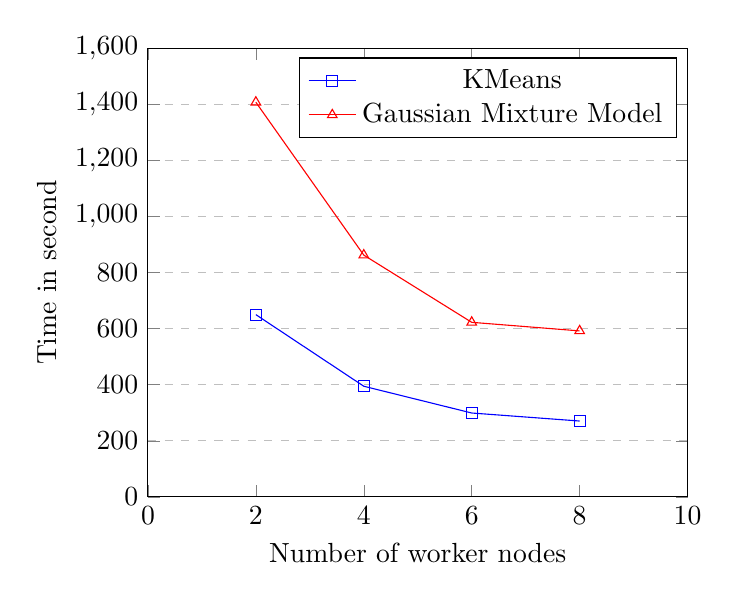
\begin{tikzpicture}
\begin{axis}[
    xlabel={Number of worker nodes},
    ylabel={Time in second},
    xmin=0, xmax=10,
    ymin=0, ymax=1600,
    xtick={0,2,4,6,8,10},
    ytick={0,200,400,600,800,1000,1200, 1400, 1600},
    ymajorgrids=true,
    grid style=dashed,
]

\addlegendentry{KMeans},
\addplot[color=blue, mark=square,]
    coordinates {
    (2, 650.17) (4, 394.63) (6, 299.12) (8, 270.49)
    };

\addlegendentry{Gaussian Mixture Model}
\addplot[color=red, mark=triangle,]
    coordinates {
    (2, 1408.23) (4, 862.63) (6, 622.77) (8, 592.13)
    };
\end{axis}
\end{tikzpicture}
\end{figure}

\begin{figure}
\caption{Scalability Experiment - Scaling and Normalization}   
\label{plt:Scaling and Normalization - Scalability Experiment Result}
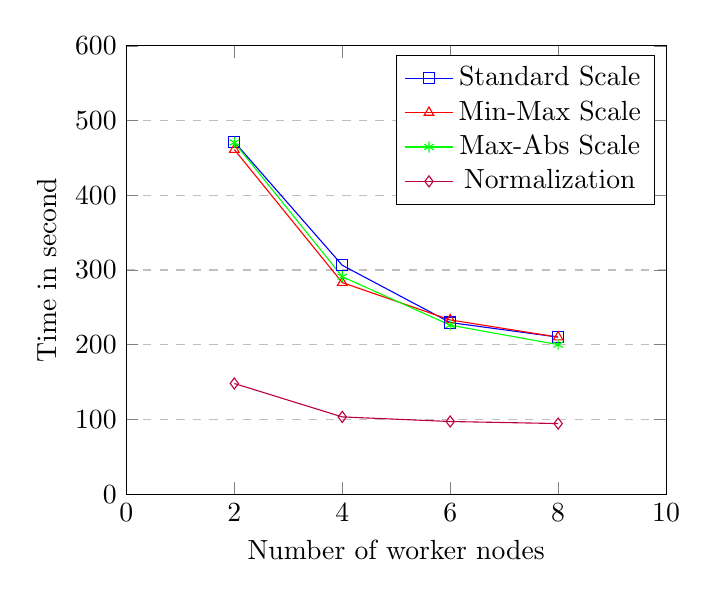
\begin{tikzpicture}
\begin{axis}[
    xlabel={Number of worker nodes},
    ylabel={Time in second},
    xmin=0, xmax=10,
    ymin=0, ymax=600,
    xtick={0,2,4,6,8,10},
    ytick={0,100,200,300,400,500,600},
    ymajorgrids=true,
    grid style=dashed,
]

\addlegendentry{Standard Scale},
\addplot[color=blue, mark=square,]
    coordinates {
    (2, 471.40) (4, 306.26) (6, 229.64) (8, 210.12)
    };

\addlegendentry{Min-Max Scale}
\addplot[color=red, mark=triangle,]
    coordinates {
    (2, 461.14) (4, 283.11) (6, 233.15) (8, 210.12)
    };

\addlegendentry{Max-Abs Scale}
\addplot[color=green, mark=asterisk,]
    coordinates {
    (2, 470.56) (4, 291.03) (6, 226.09) (8, 200.07)
    };

\addlegendentry{Normalization}
\addplot[color=purple, mark=diamond,]
    coordinates {
    (2, 148.06) (4, 103.33) (6, 97.17) (8, 94.43)
    };
\end{axis}
\end{tikzpicture}
\end{figure}

\subsubsection{Scalability} We evaluate the scalability of different functionalities of PyPandas. In our measurement, we uses the total execution times, which includes the time for Spark initialization, data loading, and data preprocessing. 

For each task, we use 4 configurations of the clusters. The 4 configurations are exactly the same, except they have different numbers of worker nodes. On each configuration, the same task is performed 3 times, and the average time consumed is record. 

From the experiment, we find that PyPandas outlier remover has great scalability. Each time we double the number of worker nodes, the performance improves significantly. Note that the improvement is not perfectly linear, because we include the spark initialization and data loading time in our measurement. As the number of workers increases, the overhead of the cluster also increases.
\begin{itemize}
	\item{Outlier Detection}: This experiment is performed on the 311 Service Requests Dataset. We perform outlier detection on one particular column that contains numerical values. We use both K-Means and Gaussian Mixture Outlier Remover with k value of 5.  The results are shown in figure \ref{plt:Outlier Detection - Scalability Experiment Result}.
	\item{Scaling and Normalization}: This experiment is performed on the 311 Service Requests Dataset. We choose all the columns containing numeric values in the dataset to do scaling and normalization. The results are shown in figure \ref{plt:Scaling and Normalization - Scalability Experiment Result}.
	\item{Text Cleaner}: This experiment is performed on the 311 Service Requests Dataset. We perform the sub\_with\_pattern function to replace all the special characters appear in the dataset with empty value. The results are shown in figure \ref{plt:Text Cleaner - Scalability Experiment Result}.
\end{itemize}

\begin{figure}
\caption{Scalability Experiment - Text Cleaner}   
\label{plt:Text Cleaner - Scalability Experiment Result}
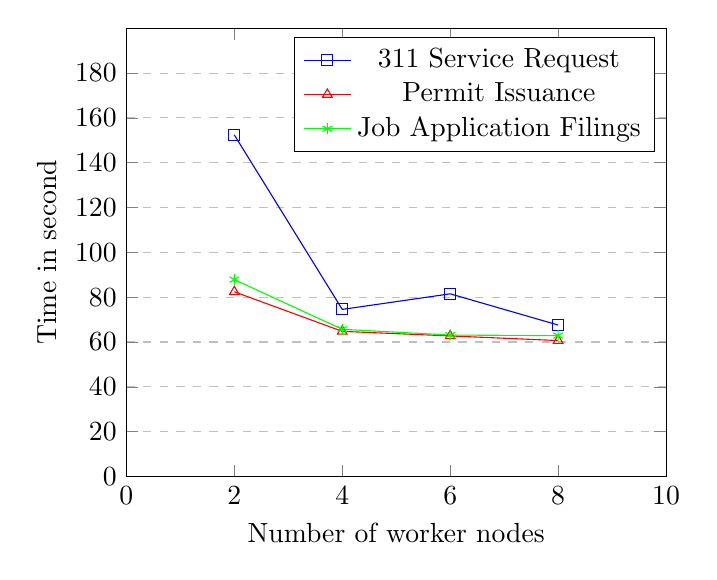
\begin{tikzpicture}
\begin{axis}[
    xlabel={Number of worker nodes},
    ylabel={Time in second},
    xmin=0, xmax=10,
    ymin=0, ymax=200,
    xtick={0,2,4,6,8,10},
    ytick={0,20,40,60,80,100,120, 140, 160, 180},
    ymajorgrids=true,
    grid style=dashed,
]

\addlegendentry{311 Service Request},
\addplot[color=blue, mark=square,]
    coordinates {
    (2, 152.39) (4, 74.56) (6, 81.51) (8, 67.59)
    };

\addlegendentry{Permit Issuance}
\addplot[color=red, mark=triangle,]
    coordinates {
    (2, 82.42) (4, 64.77) (6, 62.73) (8, 60.67)
    };

\addlegendentry{Job Application Filings}
\addplot[color=green, mark=asterisk,]
    coordinates {
    (2, 87.85) (4, 65.69) (6, 63.12) (8, 62.87)
    };
\end{axis}
\end{tikzpicture}
\end{figure}

\section{Conclusions}
Due to the lack of advanced data cleaning library on Spark ecosystem, we propose PyPandas, a data cleaning toolkit built on PySpark. We provide useful advanced data cleaning features such as outlier detection, data scaling, and text pattern searching and replacement. The library is easy to install and has user friendly APIs. PyPandas also has good performance and scalability.

%\section{reference}
\bibliographystyle{ACM-Reference-Format}
\bibliography{citation}


\end{document}
